%------------------------------------------------------------------------

\chapter[The ordinal epsilon0]{The Ordinal  \texorpdfstring{$\epsilon_0$}{Epsilon0}}

\label{cnf-math-def}
\label{chap:T1}

In this chapter, we adapt to \coq{} the well-known proof~\cite{KP82} that Hercules eventually wins every battle, whichever the strategy  of each player.
In other words, we present  a formal and self-contained proof of termination  of all [free] hydra battles.
First, we take from Manolios and Vroon~\cite{Manolios2005} a representation of the ordinal $\epsilon_0$ as terms in Cantor normal form. Then, we define a variant for hydra battles as a measure that maps any hydra to some ordinal strictly less than $\epsilon_0$.



\section{The ordinal \texorpdfstring{\(\epsilon_0\)}{epsilon0}}
\label{sec:epsilon0-intro}

The ordinal \(\epsilon_0\) is the least ordinal number that satisfies 
the equation \(\alpha = \omega^\alpha\), where \(\omega\) is 
the least infinite ordinal\footnote{For a precise ---\,\emph{i.e.} mathematical\,--- definition of $\omega^\alpha$, please see Sect.~\vref{sect:AP-and-phi0}.} .
Thus, we can intuitively consider \(\epsilon_0\) as an
\emph{infinite} \(\omega\)-tower.


\subsection{Cantor normal form}
\index{maths}{Cantor normal form}



Any ordinal strictly less that \(\epsilon_0\) 
can be finitely represented by a unique  \emph{Cantor normal form}, 
that is, an expression  which is 
a sum  \(\omega^{\alpha_1} \times n_1 + \omega^{\alpha_2} \times n_2 + 
  \dots + \omega^{\alpha_p} \times n_p\) where $p\in\mathbb{N}$, all the \(\alpha_i\) 
are ordinals in Cantor  normal form, \(\alpha_1 > \alpha_2 > \alpha_p\)
and all the \(n_i\) are positive integers.

An example of Cantor normal form is displayed in Fig \ref{fig:cnf-example}:
Note that  any ordinal of
the form \(\omega^0 \times i + 0\) is just written \(i\).

\begin{figure}[htb]
\centering
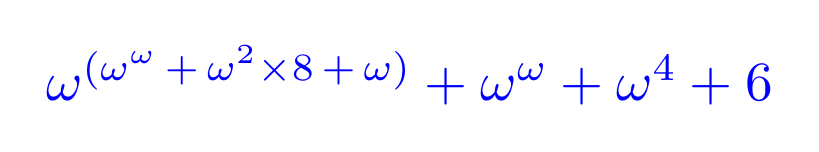
\begin{tikzpicture}[scale=2, every node/.style={transform shape}]
\node[color=blue]{$\omega^{(\omega^\omega\,+\, \omega^2 \times 8 \,+\, \omega)}+ \omega^\omega + \omega^4+ 6$};
\end{tikzpicture}
\caption{\label{fig:cnf-example}
An ordinal in Cantor normal form}
\end{figure}




In the rest of this section, we define an inductive type for representing in \texttt{Coq}
all the ordinals strictly  less than  \(\epsilon_0\), then extend some arithmetic operations
to this type, and finally prove that our representation fits well with 
the expected mathematical properties: the order we define is a well order, 
and the decomposition into Cantor normal form  is consistent 
with usual definition of ordinals, for instance in \gaia~\cite{Gaia}, Schütte's book~\cite{schutte}, or larger ordinal notations~\vref{chap:gamma0}.

\paragraph*{Remark}
\label{sec:orgheadline65}
Unless explicitly mentioned, the term ``ordinal" will be used instead of
``ordinal strictly less than \(\epsilon_0\)" (except in Chapter~\ref{chap:schutte} where it stands for ``countable ordinal'').



\subsection{A data type for  ordinals in Cantor normal form}
\label{sec:orgheadline72}
\label{sec:T1-inductive-def}



% Our user contribution~\cite{CantorContrib} represents 
% the set of ordinals strictly less than $\epsilon_0$ in Cantor normal form as in~\cite{Manolios2005}, and also the set
% of ordinals strictly  less than $\Gamma_0$ in Veblen normal form.


    Let us define an inductive type whose 
constructors are respectively associated
with the ways to build Cantor normal forms:

\begin{itemize}
\item the ordinal \(0\)
\item the construction \((\alpha,\, n,\,\beta)  \mapsto \omega^\alpha \times (n + 1)+ \beta \quad (n\in\mathbb{N})\)
\end{itemize}


\vspace{4pt}
\noindent\emph{From Module~\href{../theories/html/hydras.Epsilon0.T1.html\#T1}{Epsilon0.T1}}

\label{types:T1}
%\index{Constants!zero:T1}
\index{hydras}{Library Epsilon0!Types!T1}

\input{movies/snippets/T1/T1Def}

\subsubsection{Example}

\label{alpha0-def}
For instance, the ordinal  $\omega^\omega+\omega^3\times 5+2$ is represented by the following term of type \texttt{T1}:



\input{movies/snippets/T1/alpha0}

\begin{figure}[htb]
\centering
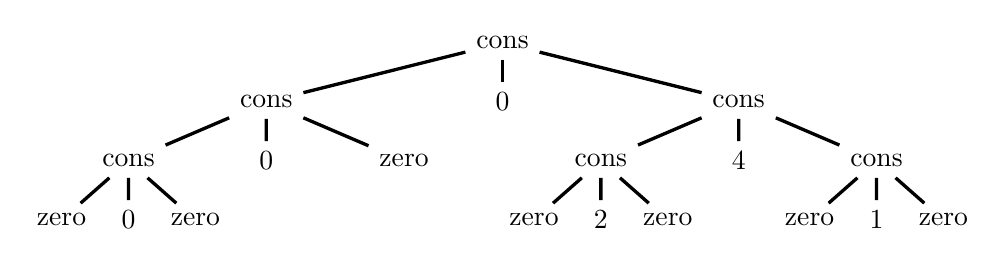
\begin{tikzpicture}[very thick, scale=0.5, level 1/.style={sibling distance=6cm},
level 2/.style={sibling distance=35mm},  
level 3/.style={sibling distance=17mm}]
\node  {cons}
  child {  node {cons}
            child { node {cons} child {node {zero}} child {node{0}} child{node{zero}}}
         child {node {0}}
         child {node {zero}}}
    child {node {0}}
   child {node {cons} 
 child { node {cons} child {node {zero}} child {node{2}} child{node{zero}}}
  child {node {4}}
         child {node {cons} child {node {zero}} child {node{1}} child{node{zero}}}};

\end{tikzpicture}

\caption{The tree-like representation of the ordinal $\omega^\omega+\omega^3\times 5 +2$\label{fig:cnf-tree}}

\end{figure}



\paragraph{Remark}
For simplicity's sake, we chose to forbid  expressions of the form $\omega^\alpha\times 0 + \beta$. Thus, the construction (\texttt{cons $\alpha$ $n$ $\beta$}) is intended to represent the
ordinal $\omega^\alpha\times(n+1)+\beta$ and not $\omega^\alpha\times n+\beta$.
In a future version, we would like to replace  the type \texttt{nat} with standard library's type \texttt{positive} in \texttt{T1}'s 
definition. But this replacement would take a lot of time \dots{}


\paragraph{Remark}
The name \texttt{T1} we gave to this data-type  is proper to this development and refers
to a hierarchy of ordinal notations. For instance, in Library \href{../theories/html/hydras.Gamma0.T2.html}{Gamma0.T2},  the following type is used to represent ordinals strictly less than \(\Gamma_0\),  in Veblen normal form (see also~\cite{Gaia, schutte}).
\noindent

\input{movies/snippets/T2/T2Def}


\subsection{About Gaia}
\index{gaiabridge}{Introduction}
\gaiasign Chapter~\vref{gaia-chapter} describes the present state of a
project of making compatible the libraries \HydrasLib and \gaia. At present, both libraries contain their own version of the inductive type \texttt{T1}, with the same base name for the constructors.

\inputsnippets{nfwfgaia/T1def}

Thus, many examples of this and following chapters can be run
in \gaia's context. We will signal any difference (notation, name) which may appear.
A closer integration (same data type and functions) is still in project.

\begin{remark}
  \label{remark:hydra-gaia-renaming}
  \textcolor{lookcolor}{In future releases, we plan to make some
    \HydrasLib identifiers progressively  deprecated, in favour of \gaia's names.}
\end{remark}



\subsection{Abbreviations}

Some abbreviations may help to write more concisely complex ordinal terms.

\subsubsection{Finite ordinals}
\label{sec:orgheadline67}

For representing finite ordinals, \emph{i.e.} natural numbers, we first introduce a notation for terms of the form $n+1$, then define a coercion from type \texttt{nat} into \texttt{T1}.
\label{sect:notation-FS}

\label{sect:notation-F}

\input{movies/snippets/T1/finiteOrds}
\index{gaiabridge}{Finite ordinals}
\paragraph*{\gaiasign}
  In \texttt{gaia.ssete9}, the $n$-th finite ordinal is also written
  \texttt{$\backslash${F}\,$n$}. There is no coercion in \gaia from \texttt{nat} to \texttt{T1}.

  \vspace{4pt}
  
  From~\href{../theories/html/gaia_hydras.HydraGaia_Examples.html}{gaia\_hydras.HydraGaia\_Examples}.

  
  \inputsnippets{HydraGaia_Examples/Demoa}


% \index{Coq!Coercions}
% \index{Functions!Coercions@Coercions (from nat to ordinal types)}
% \begin{remark}
% Please refer to the remark~\pageref{warning:coercions} about the use of coercions.
% % The use of coercions like \texttt{fin} allow us to be close to the mathematical tradition where natural numbers are ordinals too.
% % Nevertheless, it may happen that a goal like \texttt{3 < 5} could be 
% % interpreted as \texttt{(lt (fin 3) (fin 5))},  depending on the current notation scope.  
% % When this misinterpretation happens, tactics like \texttt{auto with arith}, \texttt{lia} do not work!
% % Thus, it is useful to write \texttt{(3 < 5)\%nat}  an inequality between two natural numbers. 
% \end{remark}


\subsubsection{The ordinal \(\omega\)}
\label{sec:orgheadline68}

  Since \(\omega\)'s Cantor normal form is
i.e. \(\omega^{\omega^0}\times 1+ 0\), we can define the following abbreviation:

\label{sect:omega-notation2}

\input{movies/snippets/T1/omegaDef}

Note that \texttt{T1omega} is not an identifier in \HydrasLib, thus any tactic like \texttt{unfold T1omega} would fail.

\index{gaiabridge}{The ordinal $\omega$}
\paragraph*{\gaiasign}
In \texttt{gaia.ssete9}, the ordinal $\omega$ is bound to the \emph{constant}  \texttt{T1omega} (not a notation).



\subsubsection{The ordinal \(\omega^\alpha\), a.k.a. \(\phi_0(\alpha)\)}
\label{sect:notation-phi0}
We provide also a notation for ordinals of the form $\omega^\alpha$.

\index{hydras}{Library Epsilon0!Notations!phi0@phi0 (exponential of base omega)}


\input{movies/snippets/T1/phi0Def}

\index{maths}{Additive principal ordinals}

\begin{remark}
\label{sec:orgheadline69}
The name \(\phi_0\)
   comes from ordinal numbers theory. In~\cite{schutte}, Schütte defines 
$\phi_0$  as the ordering (\emph{i.e.} enumerating) function of the set  of \emph{additive principal ordinals} \emph{i.e.} strictly positive ordinals $\alpha$ that verify $\forall \beta<\alpha, \beta+\alpha=\alpha$. For Schütte,  $\omega^\alpha$ is just a notation for $\phi_0(\alpha)$.  See also Chapter~\ref{chap:schutte} of this document.
\end{remark}

\paragraph*{\gaiasign}
\index{gaiabridge}{Exponential of base $\omega$}
In \texttt{gaia.ssete9} the identifier \texttt{phi0} is bound to a plain constant (not a notation).

  
\subsubsection{The hierarchy of \(\omega\)-towers:}
\label{sec:orgheadline71}

The ordinal $\epsilon_0$, although not represented by a finite term in Cantor normal form, is approximated by the sequence of $\omega$-towers (see also Sect~\vref{sect:epsilon0-as-limit} ).

\vspace{4pt}
\emph{From Module~\href{../theories/html/hydras.Epsilon0.T1.html}{Epsilon0.T1}}

\input{movies/snippets/T1/towerDef}


For instance, Figure~\ref{fig:tower7} represents  the ordinal returned by the
 evaluation of the term \texttt{omega\_tower 7}.

\begin{figure}[htb]
\centering
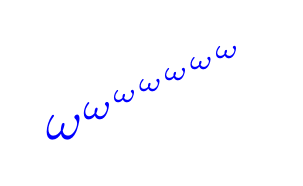
\begin{tikzpicture}[scale=2, every node/.style={transform shape}]
\node[color=blue]{$\omega^{{{\omega}^{{{\omega}}^{{{\omega}}^{{\omega^{{\omega}^{\omega}}}}}}}}$};
\end{tikzpicture}
\caption{\label{fig:tower7}
The $\omega$-tower of height 7}
\end{figure}

\subsection{Pretty-printing ordinals in Cantor normal form}
\label{sect:ppT1}
\index{hydras}{Library Epsilon0!Types!ppT1}

Let us consider again the ordinal $\alpha_0$ defined in section~\vref{alpha0-def}. 
If we ask \coq{} to print its  normal form, we get a hardly readable term of type \texttt{T1}.

\input{movies/snippets/T1/alpha0Compute}

The following data type defines a more readable abstract syntax for  ordinals terms in Cantor normal form:

\label{types:ppT1}
\index{hydras}{Library Epsilon0!Functions!pp@ pp (pretty printing terms in Cantor normal form)}

\input{movies/snippets/T1/ppT1Def}


The function \texttt{pp: T1 -> ppT1} converts any closed term of type \texttt{T1} into a human-readable expression. For instance, let us convert the term \texttt{alpha\_0}.

\input{movies/snippets/T1/ppAlpha0}

\paragraph*{\gaiasign}
\index{gaiabridge}{Pretty printing Cantor normal forms}
In ~\href{../theories/html/gaia.T1Bridge.html}{gaia.T1Bridge},
we define a variant of \texttt{pp} for pretty-printing terms of type \texttt{ssete9.CantorOrdinal.T1} (see Sect.~\vref{sect:gaia-ppT1}).

\index{hydras}{Projects}
\begin{project}
Design tools for systematically pretty printing ordinal terms in Cantor normal form.
\end{project}


\subsection{Comparison between ordinal terms}
\label{sec:orgheadline73}


% Our formalisation of Cantor Normal Form will take two steps:
% 1 Definition of a strict order \texttt{o<} on the type \texttt{T1}, 
% 2 Using \texttt{o<} for characterizing terms in normal form.

In order to compare two terms of type \texttt{T1}, we define a recursive function \texttt{compare} that maps two ordinal tems $\alpha$ and $\beta$ to a value of type \texttt{comparison}. This type is defined in \coq's standard library 
\texttt{Init.Datatypes} and
contains three constructors:  \texttt{Lt} (less than), \texttt{Eq} (equal), and
\texttt{Gt} (greater than).


\vspace{4pt}
\emph{From Module~\href{../theories/html/hydras.Epsilon0.T1.html\#compare}{Epsilon0.T1}}

\input{movies/snippets/T1/compareDef}

\input{movies/snippets/T1/Instances}


\label{Predicates:lt-T1}
Please note that this definition of \texttt{lt} makes it easy to write proofs by computation, as shown by the following examples.

\vspace{4pt}


\input{movies/snippets/T1/ltExamples}


% Links between the function \texttt{compare} and the relations
% \texttt{lt} and \texttt{eq} are established through the following lemmas (~\vref{sect:comparable-def}).
% \vspace{4pt}



\paragraph*{\gaiasign}
\index{gaiabridge}{Strict order on ordinals below $\epsilon_0$}

In \gaia, the strict order \texttt{T1lt} on ordinal terms is directly defined as a boolean function (in \ssreflect's style).

\inputsnippets{nfwfgaia/T1ltDef}

In section~\vref{sect:lt-compat-gaia}, we show that both definitions are mutually equivalent.

\subsubsection{A Predicate for Characterizing Normal Forms}
\label{sect:t1-nf}

\label{sec:orgheadline74}
\label{sec:orgheadline75}
Our data-type \texttt{T1} allows us to write expressions that
are not properly in Cantor normal form as specified in Section \ref{sec:epsilon0-intro}.
For instance, consider the following term of type  \texttt{T1}. 


\input{movies/snippets/T1/badTerm}


This term would have been written \(\omega^1\times 2 + \omega^\omega \times 3\) in the usual mathematical notation. We note that the exponents of $\omega$ are not in the right (strictly decreasing) order. The following boolean function determines whether a given ordinal term is well formed.


\vspace{4pt}
\noindent
\emph{From Module~\href{../theories/html/hydras.Epsilon0.T1.html\#nf_b}{Epsilon0.T1}}

\label{Predicates:nf-T1}


\input{movies/snippets/T1/nfDef}

\input{movies/snippets/T1/nfAlpha0}

\input{movies/snippets/T1/nfBadTerm}

\paragraph*{\gaiasign}
\index{gaiabridge}{Ordinal terms in Cantor normal form}
In \gaia, the boolean function which characterizes ordinal terms in normal form is defined as follows:

\inputsnippets{nfwfgaia/T1nfDef}

In Sect.~\vref{nf-gaia-compat}, we show that \gaia's \texttt{T1nf} is extensionally equivalent with \HydrasLib'  \texttt{nf}.



\subsection{Making normality implicit}
  We would like to get rid of terms of type \texttt{T1} which are not in Cantor normal form.
A simple way to do this is to consider statements of the form 
\texttt{forall alpha: T1, nf alpha -> $P$ alpha}, where $P$ is a predicate over type \texttt{T1}, like in the following lemma \footnote{Ordinal addition is formally defined a little later (page~\ref{sect:infix-plus-T1})}.

\input{movies/snippets/T1/plusIsZero}

\vspace{4pt}


But this style leads to clumsy statements, and generates too many subgoals in interactive proofs (although often solved with \texttt{auto} or \texttt{eauto}).

One may encapsulate conditions of the form \texttt{(nf $\alpha$)} in
the most used predicates. For instance, we introduce the restriction of \texttt{lt} to terms in normal form, and provide a handy notation for this restriction.

\vspace{4pt}
\emph{From Module~\href{../theories/html/hydras.Prelude.Restriction.html}{hydras.Prelude.Restriction}}

\input{movies/snippets/Restriction/restrictionDef}

\vspace{4pt}
\emph{From Module~\href{../theories/html/hydras.Epsilon0.T1.html\#LT}{Epsilon0.T1}}

\input{movies/snippets/T1/LTDef}

\label{Predicates:LT-T1}
 

For instance, in the following lemma, the condition that $\alpha$ is in normal form is included in the condition $\alpha< 1$.

\input{movies/snippets/T1/LTOne}


\subsubsection{\texttt{E0}: a sigma-type for \texorpdfstring{$\epsilon_0$}{epsilon0}}

As we noticed in Sect.~\ref{sect:t1-nf}, the type \texttt{T1} is not a correct ordinal notation, since it contains terms that are not in Cantor normal form. In certain contexts (for instance in Sections~\ref{sect:L-equations}, \ref{sect:hardy},
and \ref{sect:wainer}),  we need to define total recursive functions on well-formed ordinal terms less  than $\epsilon_0$, using the \texttt{Equations} plug-in~\cite{sozeau:hal-01671777}.
 In order to define a type whose inhabitants represent just ordinals, we build a type gathering a term of type \texttt{T1} and a proof that this term is in normal form.

 

 

\label{sect:E0-def}
\label{types:E0}
\index{hydras}{Library Epsilon0!Types!E0}

\emph{From Module~\href{../theories/html/hydras.Epsilon0.E0.html\#E0}{Epsilon0.E0}}

\input{movies/snippets/E0/E0Def}


Many constructs : types, predicates, functions, notations, etc., on type \texttt{T1} are adapted to \texttt{E0}.

First, we declare a notation scope for \texttt{E0}, then we redefine the predicates of comparison.


\input{movies/snippets/E0/E0Scope}
\label{Predicates:Lt-E0}
\input{movies/snippets/E0/LtLeDef}




Equality in \texttt{E0} is just Leibniz equality. Note that, since \texttt{nf} is
defined by a Boolean function, for  any term $\alpha:\texttt{T1}$, there exists at most one proof of \texttt{nf $\alpha$}, thus two ordinals of type \texttt{E0} are
equal if and only if their projection to \texttt{T1} are equal (see also Sect.~\vref{sect:eq-proof-unicity}).

\vspace{4pt}


\index{coq}{Unicity of equality proofs}

\inputsnippets{E0/nfProofUnicity}
\inputsnippets{E0/E0EqIff}


In order to  upgrade constants and functions from type \texttt{T1} to \texttt{E0}, we have to prove that
the term they build is in normal form.
For instance, let us represent the ordinals $0$ and $\omega$   as instances of the class \texttt{E0}.

\vspace{4pt}

\label{sect:omega-T1}

\input{movies/snippets/E0/ZeroOmega}

%\index{Constants!zero:T1}

\paragraph*{\gaiasign}
\index{gaiabridge}{Type of well formed ordinal terms below $\epsilon_0$}
 Our library~\href{../theories/html/gaia_hydras.T1Bridge.html}{gaia\_hydras.T1Bridge} also defines a type \texttt{E0} (which doesn't exist in \gaia-\texttt{ssete9}). 



\subsection{Syntactic definition of limit and successor ordinals}

Pattern matching and structural recursion allow us to define boolean characterizations  of successor and limit ordinals.


\vspace{4pt}
\noindent
\emph{From Module~\href{../theories/html/hydras.Epsilon0.T1.html\#T1is_succ}{Epsilon0.T1}}



\input{movies/snippets/T1/succbLimitb}


The correctness of these definitions with respect to the mathematical notions of
limit and successor ordinals is established through several lemmas. For instance,
Lemma \texttt{canonS\_limit\_lub}, page~\pageref{lemma:canonS-limit}, shows that
if $\alpha$ is (syntactically) a limit ordinal, then it is the least upper bound of
a strictly increasing sequence of ordinals.


\paragraph*{\gaiasign}
\index{gaiabridge}{Limit and successor ordinals}
In \gaia, the boolean functions associated with limit and successor ordinals are also called \texttt{T1limit} and \texttt{T1is\_succ}.

 From~\href{../theories/html/gaia_hydras.HydraGaia_Examples.html}{gaia\_hydras.HydraGaia\_Examples}.

  
\inputsnippets{HydraGaia_Examples/Demob}





\subsection{Arithmetic on \texorpdfstring{$\epsilon_0$}{epsilon0}}
\subsubsection{Successor}

\index{hydras}{Library Epsilon0!Functions!succ}

The successor of any ordinal $\alpha< \epsilon_0$ is defined by structural 
recursion on its Cantor normal form.

\label{Functions:succ-T1}

\vspace{4pt}
\noindent
\emph{From Module~\href{../theories/html/hydras.Epsilon0.T1.html\#succ}{Epsilon0.T1}}


\input{movies/snippets/T1/succDef}

The following lemma establishes the connection between the  function
\texttt{succ} and the Boolean predicate \texttt{T1is\_succ}.

\vspace{4pt}

\input{movies/snippets/T1/succbIff}

\begin{exercise}
  \gaiasign Look for the \gaia-theorem which corresponds to \texttt{T1is\_succ\_iff}.
\end{exercise}

\subsubsection{Successor function on \texttt{E0}}

The function \texttt{succ} on \texttt{T1} is extended to \texttt{E0} the following way:

 \emph{From Module~\href{../theories/html/hydras.Epsilon0.E0.html}{Epsilon0.E0}}

 \inputsnippets{E0/SuccOnE0}

 
\index{hydras}{Exercises}
 \begin{exercise}
Prove in \coq{} that for any ordinal $0< \alpha<\epsilon_0$, $\alpha$ is a limit if 
and only if for all $\beta<\alpha$, the interval $[\beta,\alpha)$ is
infinite.

\emph{You may start this exercise with the file
     \href{https://github.com/coq-community/hydra-battles/tree/master/exercises/ordinals/Limit_Infinity.v}{exercises/ordinals/Limit\_Infinity.v}.}
 \end{exercise}

 
  
\subsubsection{Addition and multiplication}

Ordinal addition and multiplication are also defined by structural recursion over the type \texttt{T1}. Please note that they use the \texttt{compare} function on some subterms of their arguments.

\label{sect:infix-plus-T1}

\input{movies/snippets/T1/plusDef}

\input{movies/snippets/T1/multDef}

\paragraph*{\gaiasign}
We keep \gaia's base names for
addition and multiplication of ordinal terms below $\epsilon_0$.
Please refer to Sect.~\ref{sect:plus-mult-gaia-hydras} about compatibility of both arithmetics.

\subsubsection{Examples}

The following examples are instances of \emph{proofs by computation}. Please note that  addition and multiplication on \texttt{T1}
are not commutative. Moreover,  both operations fail to be strictly monotonous in their first argument.

\input{movies/snippets/T1/plusMultExamples}

\input{movies/snippets/T1/notMono}


The function \texttt{succ} is related with addition through the following lemma:

\inputsnippets{T1/succIsPlusOne, T1/succIsPlusOnez}



\subsubsection{Arithmetic on type \texttt{E0}}

 We define an addition in type \texttt{E0}, since the sum of two terms in normal form is in normal form too.

\input{movies/snippets/T1/plusNf}

\input{movies/snippets/E0/plusE0}
\input{movies/snippets/E0/CheckPlus}


\begin{remark}
In all this development, two representations of ordinals co-exist: ordinal terms (type \texttt{T1}, notation scope \texttt{t1\_scope}, for reasoning on the tree-structure of Cantor normal forms), and ordinal terms \emph{known to be in normal form} (type \texttt{E0}, notation scope \texttt{E0\_scope}). Looking at the contexts displayed by \coq{} prevents you from any risk of confusion.
\end{remark}

%% To simplify !
\index{hydras}{Exercises} 
\begin{exercise}
Prove that for any ordinal $\alpha:\texttt{E0}$, 
$\omega\leq \alpha$ if and only if, for any natural number $i$,
$i+\alpha=\alpha$.

\emph{You may start this exercise with the file
    \href{https://github.com/coq-community/hydra-battles/tree/master/exercises/ordinals/ge_omega_iff.v}{exercises/ordinals/ge\_omega\_iff.v}.}
\end{exercise}

\subsection{A proof by computation}
\label{Ex42-E0}

It is interesting to compare the following proof of the equality
$\omega+42+\omega^2$ with the more theoretical proof in Sect~\vref{Ex42-schutte}.

\inputsnippets{E0/Ex42}

\section{Well-foundedness and transfinite induction}

\index{maths}{Transfinite induction}

\subsection{About  well-foundedness}
\label{sec:T1Wf}
\label{sec:orgheadline82}
   In order to use \texttt{T1} for proving termination results,
we need to prove that  our order \texttt{<} is well-founded. Then we will get \emph{transfinite induction} for free.


The proof of well-foundedness of the strict order $<$ on Cantor normal forms is already 
available in the Cantor contribution by Castéran and Contejean~\cite{CantorContrib}. That proof relies on a library on recursive path orderings written by
E. Contejean. We present here  a direct proof of the same result, which does not require any knowledge on r.p.o.s.

\index{hydras}{Exercises}

\begin{exercise}
Prove that the \emph{total} order \texttt{lt} on \texttt{T1} is not well-founded. 
\textbf{Hint:}  You will have to build a counter-example with terms of type \texttt{T1}
which are not in Cantor normal form.

\emph{You may start this exercise with the file
    \href{https://github.com/coq-community/hydra-battles/tree/master/exercises/ordinals/T1_ltNotWf.v}{exercises/ordinals/T1\_ltNotWf.v}.}
\end{exercise}

\subsubsection{A first attempt}
\label{sec:orgheadline77}
%\index{coq}{Well-founded induction}

It is natural to try to prove by structural induction over \texttt{T1} 
that every term in normal form is \texttt{LT}-accessible.

Unfortunately, it won't work. Let us consider some well-formed term
 $\alpha=\texttt{cons $\beta\;n\;\gamma$}$, and assume that \(\beta\) and \(\gamma\) are \texttt{LT}-accessible.
In order to prove the accessibility of $\alpha$, we have to consider
any well formed term \(\delta\) such that \(\delta<\alpha\). 
% But nothing guarantees that \(\delta\)  is strictly  less than \(\beta\) nor \(\gamma\), and we cannot use the induction hypotheses on   \(\beta\) nor \(\gamma\).

\input{movies/snippets/T1/wfLTBada}


The problem comes from the too weak hypothesis \texttt{Hdelta}. It does not prevent  \(\delta\) to be bigger that \(\beta\) or
\(\gamma\);
for instance \(\delta\) may be of the form
\texttt{cons $\beta$ $p'$  $\gamma'$},
where    \(p' < n\).
Thus, the induction hypotheses \texttt{IHbeta} and \texttt{IHgamma}  are useless for finishing our proof.

\input{movies/snippets/T1/wfLTBadz}

\subsubsection{Using a stronger inductive predicate.}
\label{sec:orgheadline78}
\label{sec:strongly-accessible}

  Instead of trying to prove directly that any ordinal term \(\alpha\) in normal form is accessible
through \texttt{LT}, we propose to consider the following (stronger) predicate:

\input{movies/snippets/T1/AccStrongDef}


The following lemma is an application of the strict inequality 
$\alpha < \omega ^\alpha$. If $\alpha$ is strongly accessible, then, by definition,
$\omega^\alpha$ is accessible, thus $\alpha$ is \emph{a fortiori} accessible.

\input{movies/snippets/T1/AccStrongStronger}


Thus, it remains to prove that every ordinal strictly less than $\epsilon_0$
is strongly accessible.

% \subsubsection{Structure of the proof of well-foundedness of \texttt{LT}}

\label{sec:orgheadline81}
\label{proof-wf-epsilon0}
\paragraph{A helper}
\label{sec:orgheadline79}

First, we prove that, for  any \texttt{LT}-accessible term $\alpha$, $\alpha$ is 
strongly accessible too.
The following proof is structured as an induction on $\alpha'$s accessibility. Let us consider
any  accessible term $\alpha$.

\input{movies/snippets/T1/AccImpAccStrong}


First, we prove that, for any $n$ and $\beta$, if (\texttt{cons $\alpha$ $n$ $\beta$}) is in normal form, then
 $\beta$ is accessible.

\inputsnippets{T1/betaAcc}

The new hypothesis  \texttt{beta\_Acc} allows us to prove by well-founded induction on $\beta$, 
and natural induction on $n$ that (\texttt{cons $\alpha$ $n$ $\beta$}) is accessible.

\inputsnippets{T1/useBetaAcc}

The proof, quite long, can be consulted in \href{../theories/html/hydras.Epsilon0.T1.html}{Epsilon0.T1}.

\paragraph{Accessibility of any well-formed ordinal term}
\label{sec:orgheadline80}

Our goal is still to prove accessibility of any well formed ordinal term.
Thanks to our previous lemmas, we are almost done (by a simple structural induction!).

\input{movies/snippets/T1/nfAcc}

\input{movies/snippets/T1/T1Wf}

\subsection{Transfinite induction}
\index{maths}{Transfinite induction}


Traditionnally, well-founded induction on ordinals is called \emph{transfinite induction}.

\inputsnippets{T1/transfiniteRecursor, T1/transfiniteInduction}

As a corollary, the order \texttt{Lt} on type \texttt{E0} is well-founded too.

\inputsnippets{E0/E0LtWf}


\begin{remark}[Related work]
\label{remark:a3pat}
A proof of well-foundedness using \'Evelyne Contejean's work on
    recursive path ordering~\cite{DershowitzRPO, a3pat} is also available in the
    library \href{../theories/html/hydras.Epsilon0.Epsilon0rpo.html}{Epsilon0.Epsilon0rpo}.

    In~\cite{Manolios2005}, Manolios and Vroom prove the well-foundedness of ordinal terms below $\epsilon_0$ by reduction to the natural order on the set of natural numbers.
 \end{remark}



\subsection{An ordinal notation for  \texorpdfstring{$\epsilon_0$}{epsilon0}}


We are now able to build an instance of \texttt{ON}.

\vspace{4pt}
\noindent
\emph{From Module~\href{../theories/html/hydras.Epsilon0.E0.html}{Epsilon0.E0}}

\input{movies/snippets/E0/InstanceEpsilon0}

\label{instance-epsilon0}


We prove also that this notation is correct w.r.t. Schutte's model (see Chapter~\ref{chap:schutte}).

\vspace{4pt}
\noindent
\emph{From Module~\href{../theories/html/hydras.Schutte.Correctness_E0.html}{Schutte.Correctness\_E0}}


\input{movies/snippets/Correctness_E0/injectDef}

\input{movies/snippets/Correctness_E0/Epsilon0Correct}


\subsection{An ordinal notation for  \gaia's ordinals}
\index{gaiabridge}{Ordinal notations}

\gaiasign Module~\href{../theories/html/gaia.T1Bridge.html}{gaia.T1Bridge} contains an instance of class \texttt{ON E0lt compare}, where \texttt{E0lt} is the order on the well-formed ordinal terms below $\epsilon_0$ defined in \gaiaHydras library (please see Chapter~\ref{gaia-chapter}).

\inputsnippets{T1Bridge/gEpsilon0}




\index{hydras}{Projects}
\begin{project}
 \emph{This exercise is a continuation of Project~\vref{exo:ON-mult}.}
Use \texttt{ON\_mult} to define an ordinal notation \texttt{Omega2} for $\omega^2=\omega\times\omega$.

Prove that \texttt{Omega2} is a sub-notation of \texttt{Epsilon0}.

Define on \texttt{Omega2} an addition compatible with the addition on \texttt{Epsilon0}.

\textbf{Hint}. You may use the following definition (in 
    \href{../theories/html/hydras.OrdinalNotations.ON_Generic.html}{OrdinalNotations.ON\_Generic}).

\input{movies/snippets/ON_Generic/SubONSameOp}
    
     \end{project}

    \index{hydras}{Projects}
    \begin{project}
    The class \texttt{ON} of ordinal notations has been defined long after this 
    chapter, and is not used in the development of the type \texttt{E0} yet.
    A better integration of both notions should simplify the development on ordinals in Cantor normal form. This integration is planned for the future versions.

    \end{project}

 

    \section{An ordinal notation for \texorpdfstring{$\omega^\omega$}{omega\^omega}}
    \label{sect:omegaomega}
    
    In Module   \href{https://github.com/coq-community/hydra-battles/blob/master/theories/
      ordinals/OrdinalNotations/OmegaOmega.v}{theories/ordinals/OrdinalNotations/OmegaOmega.v},
    we represent ordinals below $\omega^\omega$ by lists of pairs of natural numbers (with the same coefficient shift as in \texttt{T1}).
    For instance, the ordinal $\omega^4\times 10 + \omega^3 + \omega+ 5$ is represented by the list \texttt{(4,9)::(3,0)::(1,0)::(0,4)::nil}.

\inputsnippets{OmegaOmega/LODef}
    
    
  The usual operations : \texttt{succ}, \texttt{+}, \texttt{*} are simple variants of the same operations in \texttt{T1}.

  \inputsnippets{OmegaOmega/succPlusMult}
  
    We establish this representation as a \emph{refinement} of the data types we used to represent ordinals less than $\epsilon_0$. Thus, many properties like well-foundedness of $<$ and associativity of $+$,  of this ordinal notations have very short proofs.

    \inputsnippets{OmegaOmega/refineDef, OmegaOmega/phi0Ref,
      OmegaOmega/succRef, OmegaOmega/plusRef,
      OmegaOmega/multRef}

    In order to make an ordinal notation for $\omega^\omega$, we follow the same steps as for $\epsilon_0$:
    \begin{enumerate}
    \item Define an order \texttt{lt}, which refines the order
      \texttt{lt} on \texttt{T1}.
      \inputsnippets{OmegaOmega/compareDef}
      \inputsnippets{ OmegaOmega/ltDef, OmegaOmega/ltRef}
      
    \item Define the predicate ``to be in normal form''.
      \inputsnippets{OmegaOmega/nfDef}
    \item Define a class \texttt{OO} of terms in normal form, and an embedding from \texttt{E0} into \texttt{OO}.
      \inputsnippets{OmegaOmega/OODef}
       \inputsnippets{OmegaOmega/embedDef}
      \item Infer well-foundedness of the order on \texttt{OO}.
    \inputsnippets{OmegaOmega/ltWf} 
      
    \end{enumerate}

    \inputsnippets{OmegaOmega/ONOO, OmegaOmega/OOz}

    Let us show a few examples.
    
    \inputsnippets{OmegaOmega/OODemo}

    \index{hydras}{Exercises}


    \subsection{Related work}
    The article~\cite{Manoury2016}  defines another representation of ordinals below $\omega^\omega$ based on lists of natural numbers.


    
\begin{exercise}
  It may be interesting to write a \emph{direct} proof  of well-foundedness of the order in $\omega^\omega$ (\emph{i.e.}
  without using properties of $\epsilon_0$). This exercise may
  help to understand better the proof structure of Sect.~\vref{sec:strongly-accessible}.
    \end{exercise}
%ici
    \section{A variant for hydra battles}

    In order to prove the termination of any hydra battle, we try to define a variant mapping hydras to ordinals strictly less than $\epsilon_0$.
    In order to make such a variant easy to define (for instance by a structural recursion), we introduce a variant of addition, which, contrary to
    $+$, is commutative and strictly monotonous in both of its arguments. This last property makes it possible to prove that our function is 
    truly a variant for hydra battles (in Sect.~\vref{sect:variant-decr}).

    \subsection{Natural sum (a.k.a. Hessenberg's  sum)}
    \label{sec:orgheadline87}
    \label{hydra-variant}
    \label{sect:hessenberg-def}
    
    Natural sum (Hessenberg  sum) is a commutative and monotonous version of
    addition. It is used as an auxiliary operation  for defining variants
    for hydra battles, where Hercules is allowed to chop off any  head of the hydra.

    In the literature, the natural sum of ordinals \(\alpha\) and \(\beta\)
    is often denoted by \(\alpha \# \beta\)  or  \(\alpha \oplus  \beta\).
    Thus we called \texttt{oplus} the associated \emph{Coq} function.

    \subsubsection{Definition of \texttt{oplus}}
    \label{sec:orgheadline84}
    %\index{Functions!oplus @ oplus (Hessenberg commutative sum)}

    The definition of \texttt{oplus} is recursive in both of its 
    arguments and uses  the same pattern as for the \texttt{merge} function on lists of library
    \texttt{Coq.Sorting.Mergesort}.

    \begin{enumerate}
    \item Define a nested recursive function, using the \texttt{Fix} 
        construct

    \item Build a principle of induction dedicated to \texttt{oplus}

    \item Establish equations associated to each case of the definition.
    \end{enumerate}

    \paragraph{Nested recursive definition}
    \label{sec:orgheadline83}
    \label{sec:oplusdefT1}
    
    The following definition is composed of 
    \begin{itemize}
    \item A main function \texttt{oplus}, structurally recursive in its 
    first argument \texttt{alpha}
    \item An auxiliary function \texttt{oplus\_aux} within the scope of \texttt{alpha},
    structurally recursive in its argument \texttt{beta};  \texttt{oplus\_aux beta} 
       is supposed to compute  \texttt{oplus alpha beta}.
    \end{itemize}
      
%  \pagebreak 
  \vspace{4pt}
    \emph{From Module~\href{../theories/html/hydras.Epsilon0.Hessenberg.html\#oplus}{Epsilon0.Hessenberg}}

    \label{sect:infix-oplus}

    \input{movies/snippets/Hessenberg/oplusDef}
    
 
    The reader will note that each recursive call of the functions
    \texttt{oplus} and \texttt{oplus\_aux} satisfies \emph{Coq}'s constraint
    on recursive definitions. The function \texttt{oplus} is recursively called on a sub-term of its first argument,
    and \texttt{oplus\_aux} on a sub-term of its unique argument.
    Thus, \texttt{oplus}'s definition is accepted by \coq{} as a structurally recursive function.

    \subsubsection{Rewriting lemmas}
    \label{sec:orgheadline86}

    \emph{Coq}'s constraints on recursive definitions result in 
    the quite  complex form of \texttt{oplus}'s definition.
    Proofs of properties of this function can be simpler if we
     derive a few  rewriting lemmas that will help to simplify 
    expressions of the form (\texttt{oplus $\alpha$ $\beta$}).

    A first set of lemmas correspond to the various cases of \texttt{oplus}'s 
    definition. They can be proved almost immediately. Here are a few examples.
    

    \inputsnippets{Hessenberg/oplusNeutral,
      Hessenberg/oplusCompareLt}

   
    


    % \subsubsection{A hand-made induction principle}
    % \label{sec:orgheadline85}

    % \index{Coq!Commands!Functional Scheme}

    % \emph{Coq} contains a command  \texttt{Functional Scheme} that 
    % generates induction principles which correspond to recursive functions.
    % Unfortunately, the current version ( \texttt{8.11.0} ) doesn't work on \texttt{oplus},
    % probably because of the inner \texttt{Fix}.

    % \begin{Coqsrc}
    % Functional Scheme oplus_ind := Induction for oplus Sort Prop.
    % \end{Coqsrc}

    % \begin{Coqanswer}
    % Error: Anomaly "todo." Please report at http://coq.inria.fr/bugs/.
    % \end{Coqanswer}


    % Fortunately, it's a good exercise for a semi-experienced user, to write
    % her/him-self induction principles similar to the ones returned by
    % \texttt{Functional Scheme}.

    % \begin{itemize}
    % \item First, we choose to write a version for sort \texttt{Type}, since versions
    % for sorts \texttt{Prop} and \texttt{Set} can be easily derived from
    % the former one. According to \emph{Coq}'s naming politics, we will call our 
    % principle \texttt{oplus\_rect}

    % \item The conclusion of \texttt{oplus\_rect} will be (\texttt{$P$ a b (oplus a b)}),
    % where $P$ is an arbitrary function of type 
    % \texttt{T1 -> T1 -> T1 -> Type}

    % \item The premises of \texttt{oplus\_rect} will describe how to build an induction 
    % on the graph of \texttt{oplus}.
    % \end{itemize}

    % We are now ready to state and prove \texttt{oplus\_rect}, and the reader
    % will note that the statement is longer than the proof script itself,
    % which is a standard proof by induction, simplification and case-analysis 
    % that follows  \texttt{oplus}'s definition.

    % We associate also a tactic to the application of \texttt{oplus\_rect}.

    % \begin{Coqsrc}
    %  Lemma oplus_rect:
    %       forall P: T1 -> T1 -> T1 -> Type, 
    %         (forall a:T1, P zero a a) ->
    %         (forall a: T1, P a zero a) ->
    %         (forall a1 n1 b1 a2 n2 b2 o,
    %            compare a1 a2 = Gt ->
    %            P b1 (cons a2 n2 b2) o ->
    %            P (cons a1 n1 b1) (cons a2 n2 b2)
    %              (cons a1 n1 o)) ->
    %         (forall a1 n1 b1 a2 n2 b2 o,
    %            compare a1 a2 = Lt ->
    %            P (cons a1 n1 b1) b2 o ->
    %            P (cons a1 n1 b1) (cons a2 n2 b2) 
    %            (cons a2 n2 o)) ->
    %         (forall a1 n1 b1 a2 n2 b2 o,
    %            compare a1 a2 = Eq ->
    %            P b1 b2 o ->
    %           P (cons a1 n1 b1) (cons a2 n2 b2)
    %             (cons a1 (S (n1 + n2)%nat) o)) ->
    %          forall a b, P a b (oplus a b).
    % Proof with auto.
    %    induction a.
    %    -    intro; simpl; destruct b;auto.
    %    -   induction b.
    %        + apply X0.
    %        + case_eq (compare a1 b1).
    %          * intro Comp; unfold oplus; rewrite Comp.
    %            cbn; apply X3 ...
    %          * intro Comp; cbn; rewrite Comp; apply X2...
    %          * intro Comp; cbn; rewrite Comp ...
    %  Defined.


    % Ltac oplus_induction a b:= pattern (oplus a b); apply oplus_rect.
    % \end{Coqsrc}

    % \index{Exercises}

    % \begin{exercise}
    % The induction principle \texttt{oplus\_rect} is still unused in our development. 
    % Please build some nice examples of application.
    % \end{exercise}

    \index{hydras}{Projects}
    \begin{project}
    Compare \texttt{oplus}'s definition (with inner fixpoint) with other possibilities
    (\texttt{coq-equations}, \texttt{Function}, etc.).
    \end{project}
    \subsection{More theorems on Hessenberg sum}
\index{gaiabridge}{Hessenberg sum}
    We need to prove some properties of $\oplus$, particularly about 
    its relation with the order $<$ on \texttt{T1}.

    \subsubsection{Commutativity, associativity}

    We prove  the commutativity of $\oplus$ in two steps. 
    First, we prove by transfinite induction on $\alpha$ that the restriction of $\oplus$ to the
    interval $[0,\alpha)$ is commutative.

    \index{maths}{Transfinite induction}

    \input{movies/snippets/Hessenberg/oplusComm0}

    

    Then, we infer  $\oplus$'s commutativity for any pair of ordinals:
    Let $\alpha$ and $\beta$ be two ordinals strictly less than $\epsilon_0$. Both ordinals $\alpha$ and $\beta$ are
    strictly less than $\textrm{max}(\alpha,\beta)+1$.
        Thus, we have just to apply the lemma \coqsimple{oplus\_comm\_0}.

\input{movies/snippets/Hessenberg/oplusComm}
  

    Associativity of Hessenberg sum is proved the same way.

    \input{movies/snippets/Hessenberg/oplusAssoc0}
    \input{movies/snippets/Hessenberg/oplusAssoc}
    
    
 

    \subsubsection{Monotony}

    At last, we prove that $\oplus$ is strictly monotonous in both of its arguments.

    \input{movies/snippets/Hessenberg/oplusMono}
    
      \index{hydras}{Projects}

    \begin{project}
    The library \texttt{Hessenberg} looks too long (proof scripts and compilation).
    Please try to make it simpler and more efficient!
    Thanks!
    \end{project}


    \paragraph*{\gaiasign} The module
      \href{../theories/html/gaia_hydras.~GHessenberg.html}{gaia\_hydras.GHessenberg} defines a version of Hessenberg sum
      compatible with \gaia's type \texttt{T1}.
      \index{gaiabridge}{Hessenberg sum}
    \subsection{A termination measure for hydra battles }

    \label{sec:hydra-measure}

    Let us define a measure from type \texttt{Hydra} into \texttt{T1}.


    \vspace{4pt}
    \emph{From Module~\href{../theories/html/hydras.Hydra.Hydra_Termination.html\#m}{Hydra.Hydra\_Termination}}

   \input{movies/snippets/Hydra_Termination/mDef}



    First, we prove that the measure $m(h)$  of any hydra $h$ is a well-formed ordinal term of type \texttt{T1}.

    \input{movies/snippets/Hydra_Termination/mNf}
      \input{movies/snippets/Hydra_Termination/msNf}
   
    For proving the termination of all hydra battles, we have to prove that
    \texttt{m} is a variant. First, a few technical lemmas follow the decomposition of \texttt{round} into several relations. Then the lemma \texttt{round\_decr} gathers all the cases.

    \label{sect:variant-decr}

    \input{movies/snippets/Hydra_Termination/S0Decr}
    \input{movies/snippets/Hydra_Termination/R1Decr}
    \input{movies/snippets/Hydra_Termination/S1Decr}
    \input{movies/snippets/Hydra_Termination/R2Decr}
     \input{movies/snippets/Hydra_Termination/RoundDecr}
 
      Finally, we prove termination of all (free) battles.

    \label{thm:every-battle-terminates}

    \input{movies/snippets/Hydra_Termination/FinalThm}

    \paragraph*{\gaiasign}
    \index{gaiabridge}{Termination of all hydra battles}
    The module~\href{../theories/html/gaia_hydras.GHydra.html}{gaia\_hydras.GHydra} contains a proof of \gaiaHydras version of termination of all battles.

    \inputsnippets{GHydra/mDef, GHydra/mVariant, GHydra/Termination}
    
    % \section*{Conclusion}

    % Let us recall three results we have proved so far.
    % \begin{itemize}
    % \item There exists a strictly decreasing variant which maps \texttt{Hydra} into 
    % the segment $[0,\epsilon_0)$ for proving the termination of any hydra battle
    % \item There exists \emph{no} such variant from \texttt{Hydra} into 
    % $[0,\omega^2)$, \emph{a fortiori} into $[0,\omega)$.
    % \end{itemize}

    % So, a  natural question is `` Does there exist any strictly decreasing variant mapping
    % type \texttt{Hydra} into some interval $[0,\mu)$ (where $\mu <\epsilon_0$) for proving the termination of all hydra battles''. The next chapter is dedicated to a formal proof that there exists no such $\mu$, even if we consider a restriction to the set of ``standard'' battles.






    %\include{epsilon0}


    %\include{impossibility-proofs}



